\documentclass[english]{article}

\usepackage{babel}
\usepackage{graphicx}
\usepackage{times}
\usepackage{pifont}
\usepackage[margin=1in]{geometry}
\usepackage{eurosym}
\usepackage{fancyhdr}
\usepackage[hidelinks]{hyperref}
%\usapackage{float}

\pagestyle{fancy}
\fancyhf{}


%HEADER
%**************************************************************************************
\pagestyle{fancy}
\fancyhf{}
%**************************************************************************************
\lhead{DIGITAL TELEVISION LABORATORIES WORK WITH PROMAX-4C}		 	 
\rhead{Laboratory Work in Telecommunications} 
\lfoot{EFA12SF}
\cfoot{\thepage}
\rfoot{Dmitry Boronin\\ Nikolay Arsenov\\ Alexey Tukalo}
%**************************************************************************************

\date{}
\setlength\parindent{0pt}

\begin{document}

\title{\vspace{2in}DIGITAL TELEVISION LABORATORIES WORK WITH PROMAX-4C\\
\small for Laboratory Work in Telecommunications\\
\vspace{0.5in}
\includegraphics{savonia.jpg}}

\nopagebreak
\maketitle


\vspace{3in}

\author{
\begin{flushright}
Dmitry Boronin, Nikolay Arsenov, Alexey Tukalo,\\
EFA12SF,\\
Information Technology,\\
Savonia University of Applied Sciences
\end{flushright}
}

\date{\today}
\thispagestyle{empty}

\newpage
\setcounter{page}{1}
\setcounter{tocdepth}{2}
\tableofcontents

\newpage

%MAIN CONTENT ******************************************************************************************************************
\section{Tasks}
 Explain the following definitions:
 \begin{itemize}
 \item Channel bundles (A, B, and C), DVB-T, DVB-C, DVB-S
 \item What multiplexes are shown in Kuopio (DVB-T), which channels (mid frequencies) are
they?
 \item Which is the DVB-T signal, image resolution, and what encoding it uses? Which is the
preferred signal strength (at least)?
 \item The modulation used in DVB-T, DVB-C reduction in?
 \item What it means to DVB-subtitles, whether it is in use in Finland?
 \item What it means to MHP?
 \item Which is a high-definition television, what are the concepts of HD-ready and Full HD?
 \end{itemize}
Laboratory work:
\begin{itemize}
\item User manual will help with Prolink-4C TV / Sat level meter
\item Measure the Prolink-4C level meter for DVB-T channel (A, B, and C) the signal strength
and signal, noise ratio. Make signals to the BER measurement.
\item Which channels you get the level meter display?
\item Measure the comparison, 36 analog channels (TV-2) and 49 (TV-3) for signal strength.
\item Measure the channels of the DVB-T signal strength of a spectrum analyzer.
\item Check out our i-CAN-top box (STB), which channels you will get the laboratory using an
antenna?
\end{itemize}
\section{Basic Definition}
\begin{itemize}
\item DVB- T: Digital Video Broadcast - Terrestrial is the most widely used digital television standard in use around the globe for terrestrial television transmissions. It provides many facilities and enables a far more efficient use of the available radio frequency spectrum than the previous analogue transmissions. The DVB-T transmission is capable of carrying a very significant level of data. Normally several television broadcasts may be carried on a single transmission and in addition to this several audio channels may be carried as well. As a result each transmission is called a multiplex.
\item DVB- C: The DVB-C specification was developed in 1994. It provides a toolbox of QAM modulation schemes from 16-QAM to 256-QAM for television and radio broadcasting services, as well as for data transmission. At the moment, this standard is deployed worldwide in cable systems ranging from the larger CATV networks down to smaller SMATV systems.
\item DVB- S: it describes the modulation and channel coding system for satellite digital multi programs Television (TV)/High Definition Television (HDTV) services to be used for primary and secondary distribution in Fixed Satellite Service (FSS) and Broadcast Satellite Service (BSS) bands.
\item Kuopio is now using E- multiplex with the center frequency of 730 MHz.
\end{itemize}
\section{The modulation of DVB-T and DVB-C}
\begin{itemize}
\item DVB-T: There are 3 modulation options (QPSK, 16QAM, 64QAM). There is a balance between the amount rate at which data can be transmitted and the signal to noise ratio that can be tolerated. The lower order modulation formats like QPSK do not transmit data as fast as the higher modulation formats such as 64QAM, but they can be received when signal strengths are lower.
\item DVB-C: It provides a toolbox of QAM modulation schemes from 16-QAM to 256-QAM for television and radio broadcasting services, as well as for data transmission. Recent
cable operators have already upgraded their networks, deploying 256-QAM modulation (thus achieving 50 Mbits/s payload per cable channel) and increasing the frequency range used for downstream transmission up to its maximum of 862 MHz.
\end{itemize}
\section{Multimedia Home Platform (MHP)}
\begin{itemize}
 \item MHP, or the Multimedia Home Platform, is the collective name for a compatible set of middleware specifications developed by the DVB Project. MHP was designed to work across all DVB transmission technologies. The use of an open standard for interactive TV middleware means that receiver manufacturers can target multiple markets rather than developing products to the specification of a particular broadcaster.
 \item MHP can be described as a set of instructions that tells the operating system on a digital TV receiver how to deal with an interactive TV application it has received. MHP also defines the form in which the applications are delivered at the receiver, including the service information that signals that interactive applications are present in the transport stream. (Pic. 1)
\end{itemize}
\begin{figure}
\centerline{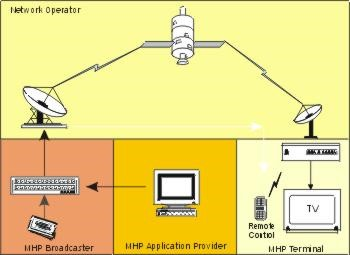
\includegraphics[scale=1]{DTV/Pic1}}
\caption{How MHP works}
\end{figure}
\section{High- Definition Television (HD- TV)}
\begin{itemize}
\item HDTV is actually part of the DTV (Digital Television) specifications, which has many different video resolutions. The two main resolutions to be concerned about are 720p and 1080i. The "p" means progressive and "i" mean interlaced. In both resolutions, every second has 60 frames of video. Progressive resolution puts 60 full frames on the screen every second. Interlaced resolution puts 30 frames of only odd lines and then 30 frames of only even lines up every second.
\item The 720p video resolution is 1280 X 720 pixels, which gives 921,600 total pixels and the 1080i video resolution is 1920 X 1080, which gives a whopping 2,073,000 pixels.
\item The term HD Ready was used in the United States to note a display that had the ability to display a high-definition picture (720p, 1080i or 1080p) but did not have a built-in HD tuner. In other words, the display worked like a monitor. It had to be connected to a set- top box or other high-definition content device that could drive a signal to it. A full HDTV was different because it had a built-in HD tuner that could receive HD over-the-air transmissions. The term HD Ready became obsolete in the United States due to FCC mandates that forced television manufacturers to include a digital tuner.
\item The term HD Ready is different in Europe. In 2005 an industry association known as EICTA (and since re-named DIGITALEUROPE) set down a standard for the term HD Ready. For a television to qualify as HD Ready it needs to be capable of 720 horizontal lines of resolution. It also must accept certain inputs such as HDMI or DVI with copy protection (HDCP). There’s also a standard called HD Ready 1080p. This standard demands that a television have native resolution of 1920×1080. It also must be able to display 1080p and 1080i video sources without overscan (in other words, the image as displayed is exactly 1920×1080) and must be able to reproduce video formats without distortion.
\item Full HD is used as a synonym for 1080p as a means of up-selling consumers looking at HD Ready sets.
\item 1080p televisions have a resolution of 1920×1080 and are progressive scan, which means all lines of each frame of video are drawn on the set. This marks 1080p as different 1080 interlaced (1080i) which alternates between rendering only the horizontal and vertical lines of each frame.
\item The difference among resolutions you can see below (Pic. 2)
\end{itemize}
\begin{figure}
\centerline{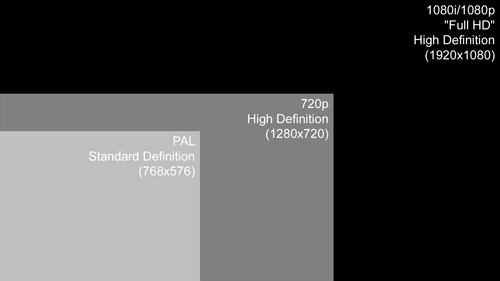
\includegraphics[scale=1]{DTV/Pic2}}
\caption{Difference among resolutions}
\end{figure}
\section{Laboratory work}
The procedure of measuring the Prolink- 4C level meter for DVB- T channel and the signal/ noise ratio.\\\\
At first, we choose the relevant measurement mode: Terrestrial band- Digital Channel. Then choose DVB-T, which obtains the error rate for the signal found in the tuned channel. After processing for a few seconds, the screen on the PROLINK-4C shows the type of modulation. We choose BER (error rate) for the digital signal after error connection. (Pic. 3)
\begin{figure}
\centerline{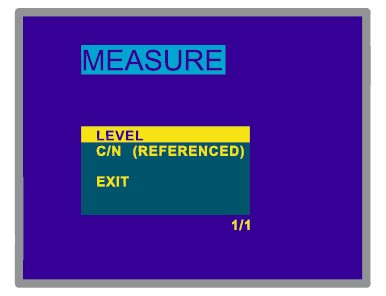
\includegraphics[scale=1]{DTV/Pic3}}
\caption{Terrestrial band- Digital Channel}
\end{figure}
There are two ways to make the measurement of the signal (noise ratio):
\begin{itemize}
\item One is automatic, in which the PROLINK- 4C defines the frequency where noise level is measured automatically. (Pic. 4)
\item The other method is defined by the users, this frequency will be used to measure noise level for all channels:
\begin{itemize}
\item Select C/N setup.
\item Turn the rotator to select C/N Auto or C/N (Reference Noise)
\end{itemize}
\end{itemize}
\begin{figure}
\centerline{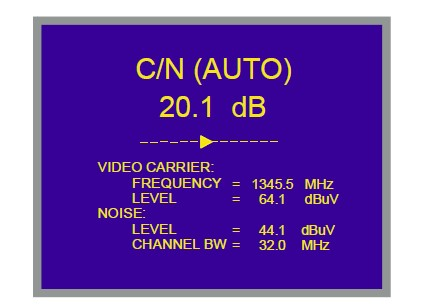
\includegraphics[scale=1]{DTV/Pic4}}
\caption{Signal and noise ration setup}
\end{figure}
\section{BER measurement mode selection}
Select the terrestrial band for the measurement of QAM or COFDM modulated signals or the satellite band for the measurement of QPSK modulated signals. Available frequency ranges are:
\begin{itemize}
\item DVB-C (QAM): 47 MHz to 862 MHz
\item DVB- T (COFDM): 40 MHz to 862 MHz
\item DVB-S (QPSK): 950 MHz to 2150 MHz
\end{itemize}
Press the rotary selector to access the COFDM signals parameters (Pic. 5) that must be defined by user:
\begin{itemize}
\item Carriers: number of modulation between 2k and 8k.
\item Guard interval: corresponds to the dead time between symbols, its purpose is to permit
a correct detection in multi- path situations. This parameter is defined according to the
symbol length: 1/4, 1/8, 1/16, 1/32.
\item Channel Bandwidth: choose between 8 MHz, 7MHz and 6 MHz
\item Spectral inversion: choose OFF position.
\item Attenuator: choose the 40 dB attenuator. Under that condition, signal level is near to
the maximum input level and it is possible that the tuner becomes saturated.
\end{itemize}
\begin{figure}
\centerline{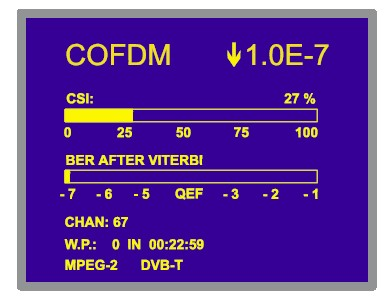
\includegraphics[scale=1]{DTV/Pic5}}
\caption{COFDM signals parameters}
\end{figure}
In a reception system of terrestrial digital signal, after the COFDM decoder two error correction methods are applied. We apply an error corrector to the digital signal, the error rate changes. (Pic. 6)
\begin{figure}
\centerline{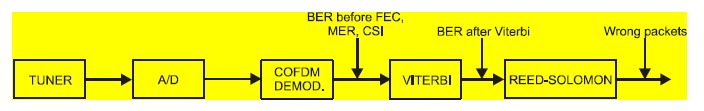
\includegraphics[scale=1]{DTV/Pic6}}
\caption{Scheme}
\end{figure}
\section{Measuring the channel of DVB- T signal strength in Spectrum Analyzer mode}
The Spectrum Analyzer mode allows the user to discover the signals present in the frequency band in quickly and easily and to make measurements at the same time. (Pic. 7)
\begin{figure}
\centerline{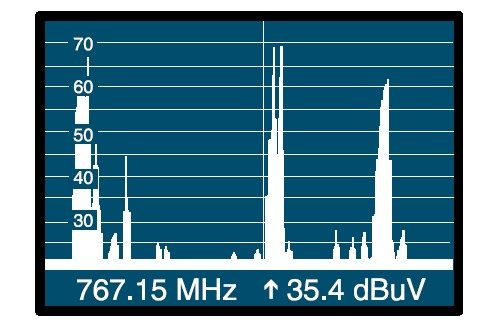
\includegraphics[scale=.8]{DTV/Pic7}}
\caption{Measurements via Spectrum Analyzer mode}
\end{figure}
The Carrier/ Noise ratio in Spectrum mode is referenced to a noise frequency defined by the user.\\\\
When measuring C/N for the digital channel in TV mode using the Auto Setup, the analogue channel may interfere in the noise measurement (formula 1) (Pic. 8):
$$
f_{noise}= f_{tuning}- \frac{1}{2} \cdot Channel Bamdwidth \;\;\;(1)
$$
\begin{figure}
\centerline{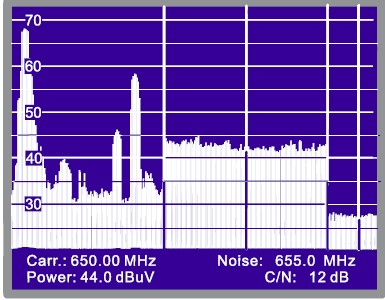
\includegraphics[scale=.8]{DTV/Pic8}}
\caption{Noise measurements}
\end{figure}
\end{document}
